%%%%%%%%%%%%%%%%%%%%%%%%%%%%%%%%%%%%%%%%%%%%%%%%%%%%%%%%%%%%
% 5.4 VECTOR CALCULUS
% The Composition of Advanced Mathematics
%%%%%%%%%%%%%%%%%%%%%%%%%%%%%%%%%%%%%%%%%%%%%%%%%%%%%%%%%%%%

\section{Vector Calculus}
\label{sec:vector-calculus}

\prerequisite{
Multivariable calculus from \cref{sec:multivariable-calculus},
single-variable calculus from \cref{sec:single-variable-calculus},
and vector and matrix ideas from \cref{sec:linear-algebra}.
}

\learningobjectives{
By the end of this section, the reader should be able to:
\begin{itemize}
    \item distinguish scalar fields from vector fields;
    \item visualize and interpret vector fields in two and three dimensions;
    \item parameterize curves and surfaces;
    \item compute tangent and normal vectors;
    \item evaluate scalar and vector line integrals;
    \item interpret line integrals as work, circulation, and accumulated density;
    \item recognize conservative vector fields;
    \item construct and use potential functions;
    \item apply the Fundamental Theorem for Line Integrals;
    \item test path independence under appropriate hypotheses;
    \item compute divergence and interpret it as local source or sink behavior;
    \item compute curl and interpret it as local rotational behavior;
    \item understand the Laplacian of a scalar field;
    \item evaluate surface integrals of scalar fields;
    \item orient surfaces and compute vector area elements;
    \item calculate flux through surfaces;
    \item apply Green's Theorem in circulation and flux forms;
    \item apply Stokes' Theorem;
    \item apply the Divergence Theorem;
    \item understand how the major integral theorems generalize the Fundamental Theorem of Calculus.
\end{itemize}
}

%%%%%%%%%%%%%%%%%%%%%%%%%%%%%%%%%%%%%%%%%%%%%%%%%%%%%%%%%%%%
\subsection{From Multivariable Calculus to Vector Calculus}
\label{subsec:from-multivariable-to-vector-calculus}
%%%%%%%%%%%%%%%%%%%%%%%%%%%%%%%%%%%%%%%%%%%%%%%%%%%%%%%%%%%%

Multivariable calculus studies scalar-valued functions such as

\[ f:\R^n\to\R. \]

Vector calculus expands this viewpoint by studying functions whose outputs
are vectors:

\[ \vect{F}:\R^n\to\R^m. \]

In physical applications, a vector field may assign a velocity, force,
electric field, magnetic field, or fluid-flow vector to every point in a
region.

For example,

\[ \vect{F}(x,y)=\langle-y,x\rangle \]

assigns a vector to each point in the plane.

\begin{conceptbox}
A scalar field assigns a number to each point. A vector field assigns a
vector to each point.
\end{conceptbox}

%%%%%%%%%%%%%%%%%%%%%%%%%%%%%%%%%%%%%%%%%%%%%%%%%%%%%%%%%%%%
\subsection{Scalar Fields}
\label{subsec:scalar-fields}
%%%%%%%%%%%%%%%%%%%%%%%%%%%%%%%%%%%%%%%%%%%%%%%%%%%%%%%%%%%%

A \emph{scalar field} is a scalar-valued function defined on a region of
space.

Examples include

\[ T(x,y,z),\qquad P(x,y,z),\qquad \rho(x,y,z). \]

These may represent temperature, pressure, and density.

For example,

\[ T(x,y)=100-x^2-y^2 \]

assigns one temperature value to each point \((x,y)\).

The gradient

\[ \nabla T \]

is then a vector field derived from the scalar field \(T\).

%%%%%%%%%%%%%%%%%%%%%%%%%%%%%%%%%%%%%%%%%%%%%%%%%%%%%%%%%%%%
\subsection{Vector Fields}
\label{subsec:vector-fields}
%%%%%%%%%%%%%%%%%%%%%%%%%%%%%%%%%%%%%%%%%%%%%%%%%%%%%%%%%%%%

\begin{definitionbox}{Vector Field}
A vector field on a region \(D\subseteq\R^n\) is a function that assigns a
vector to every point of \(D\).
\end{definitionbox}

A two-dimensional vector field has the form

\[ \vect{F}(x,y)=\langle P(x,y),Q(x,y)\rangle. \]

A three-dimensional vector field has the form

\[ \vect{F}(x,y,z)=\langle P(x,y,z),Q(x,y,z),R(x,y,z)\rangle. \]

Here \(P,Q,R\) are scalar component functions.

%%%%%%%%%%%%%%%%%%%%%%%%%%%%%%%%%%%%%%%%%%%%%%%%%%%%%%%%%%%%
\subsection{Visualizing Vector Fields}
\label{subsec:visualizing-vector-fields}
%%%%%%%%%%%%%%%%%%%%%%%%%%%%%%%%%%%%%%%%%%%%%%%%%%%%%%%%%%%%

A vector field is commonly visualized by drawing an arrow at selected
points.

The arrow indicates both:

\begin{itemize}
    \item the direction of the vector;
    \item its relative magnitude.
\end{itemize}

Consider

\[ \vect{F}(x,y)=\langle-y,x\rangle. \]

The vectors are tangent to circles centered at the origin.

\begin{center}
\begin{tikzpicture}[scale=0.85,>=stealth]
\draw[->] (-3.3,0)--(3.3,0) node[right] {$x$};
\draw[->] (0,-3.3)--(0,3.3) node[above] {$y$};

\foreach \x in {-2,-1,0,1,2}{
    \foreach \y in {-2,-1,0,1,2}{
        \pgfmathsetmacro{\u}{-0.28*\y}
        \pgfmathsetmacro{\v}{0.28*\x}
        \draw[->] (\x,\y)--++(\u,\v);
    }
}
\end{tikzpicture}
\end{center}

This is an example of a rotational vector field.

%%%%%%%%%%%%%%%%%%%%%%%%%%%%%%%%%%%%%%%%%%%%%%%%%%%%%%%%%%%%
\subsection{Radial Vector Fields}
\label{subsec:radial-vector-fields}
%%%%%%%%%%%%%%%%%%%%%%%%%%%%%%%%%%%%%%%%%%%%%%%%%%%%%%%%%%%%

Consider

\[ \vect{F}(x,y)=\langle x,y\rangle. \]

At every point, the vector points directly away from the origin.

\begin{center}
\begin{tikzpicture}[scale=0.85,>=stealth]
\draw[->] (-3.3,0)--(3.3,0) node[right] {$x$};
\draw[->] (0,-3.3)--(0,3.3) node[above] {$y$};

\foreach \x in {-2,-1,0,1,2}{
    \foreach \y in {-2,-1,0,1,2}{
        \pgfmathsetmacro{\u}{0.23*\x}
        \pgfmathsetmacro{\v}{0.23*\y}
        \draw[->] (\x,\y)--++(\u,\v);
    }
}
\end{tikzpicture}
\end{center}

Such fields appear naturally in gravitational, electric, and fluid-flow
models.

%%%%%%%%%%%%%%%%%%%%%%%%%%%%%%%%%%%%%%%%%%%%%%%%%%%%%%%%%%%%
\subsection{Vector-Valued Curves}
\label{subsec:vector-valued-curves}
%%%%%%%%%%%%%%%%%%%%%%%%%%%%%%%%%%%%%%%%%%%%%%%%%%%%%%%%%%%%

A curve in space may be represented by a vector-valued function

\[ \vect{r}(t)=\langle x(t),y(t),z(t)\rangle. \]

The bold vector \(\vect{r}\) represents the position of a moving point.

The derivative is

\[ \vect{r}'(t)=\left\langle x'(t),y'(t),z'(t)\right\rangle. \]

This vector is tangent to the curve.

If \(t\) represents time, then

\[ \vect{v}(t)=\vect{r}'(t) \]

is velocity and

\[ \vect{a}(t)=\vect{r}''(t) \]

is acceleration.

%%%%%%%%%%%%%%%%%%%%%%%%%%%%%%%%%%%%%%%%%%%%%%%%%%%%%%%%%%%%
\subsection{Parameterized Curves}
\label{subsec:parameterized-curves-vector-calculus}
%%%%%%%%%%%%%%%%%%%%%%%%%%%%%%%%%%%%%%%%%%%%%%%%%%%%%%%%%%%%

A parameterized curve in the plane may be written

\[ \vect{r}(t)=\langle x(t),y(t)\rangle,\qquad a\leq t\leq b. \]

For example,

\[ \vect{r}(t)=\langle\cos t,\sin t\rangle,\qquad0\leq t\leq2\pi \]

traces the unit circle counterclockwise.

\begin{center}
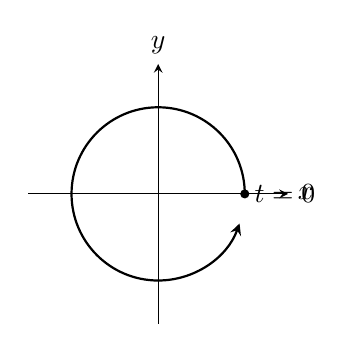
\begin{tikzpicture}[scale=1.1,>=stealth]
\draw[->] (-1.5,0)--(1.5,0) node[right] {$x$};
\draw[->] (0,-1.5)--(0,1.5) node[above] {$y$};
\draw[thick,->] (1,0) arc[start angle=0,end angle=340,radius=1];
\fill (1,0) circle (1.5pt);
\node[right] at (1,0) {$t=0$};
\end{tikzpicture}
\end{center}

%%%%%%%%%%%%%%%%%%%%%%%%%%%%%%%%%%%%%%%%%%%%%%%%%%%%%%%%%%%%
\subsection{Orientation of Curves}
\label{subsec:curve-orientation}
%%%%%%%%%%%%%%%%%%%%%%%%%%%%%%%%%%%%%%%%%%%%%%%%%%%%%%%%%%%%

A parameterization gives a curve an \emph{orientation}.

Orientation specifies the direction in which the curve is traversed.

If

\[ \vect{r}(t),\qquad a\leq t\leq b \]

traces a curve from \(A\) to \(B\), then reversing the parameterization
traces the same geometric curve from \(B\) to \(A\).

Orientation becomes essential in vector line integrals and the major
integral theorems.

%%%%%%%%%%%%%%%%%%%%%%%%%%%%%%%%%%%%%%%%%%%%%%%%%%%%%%%%%%%%
\subsection{Arc Length for Parameterized Curves}
\label{subsec:arc-length-vector-curves}
%%%%%%%%%%%%%%%%%%%%%%%%%%%%%%%%%%%%%%%%%%%%%%%%%%%%%%%%%%%%

For a smooth curve

\[ \vect{r}(t),\qquad a\leq t\leq b, \]

the differential arc length is

\[ ds=\norm{\vect{r}'(t)}\,dt. \]

Thus the total length is

\[ \boxed{L=\int_a^b\norm{\vect{r}'(t)}\,dt.} \]

The symbol

\[ ds \]

is read ``differential arc length'' or simply ``dee ess.''

%%%%%%%%%%%%%%%%%%%%%%%%%%%%%%%%%%%%%%%%%%%%%%%%%%%%%%%%%%%%
\subsection{Scalar Line Integrals}
\label{subsec:scalar-line-integrals}
%%%%%%%%%%%%%%%%%%%%%%%%%%%%%%%%%%%%%%%%%%%%%%%%%%%%%%%%%%%%

Suppose a scalar field \(f\) is defined along a curve \(C\).

The scalar line integral is

\[ \int_C f\,ds. \]

This is read:

``the line integral over \(C\) of \(f\) with respect to arc length.''

If

\[ \vect{r}(t),\qquad a\leq t\leq b \]

parameterizes \(C\), then

\[ \boxed{\int_C f\,ds
=\int_a^b f(\vect{r}(t))\norm{\vect{r}'(t)}\,dt.} \]

%%%%%%%%%%%%%%%%%%%%%%%%%%%%%%%%%%%%%%%%%%%%%%%%%%%%%%%%%%%%
\subsection{Physical Meaning of Scalar Line Integrals}
\label{subsec:scalar-line-integral-meaning}
%%%%%%%%%%%%%%%%%%%%%%%%%%%%%%%%%%%%%%%%%%%%%%%%%%%%%%%%%%%%

Suppose a thin wire follows a curve \(C\) and has linear density

\[ \rho(x,y,z). \]

Then its mass is

\[ \boxed{m=\int_C\rho\,ds.} \]

If the density is constant,

\[ \rho=\rho_0, \]

then

\[ m=\rho_0L. \]

Thus scalar line integrals generalize the familiar formula

\[ \text{mass}=(\text{density})(\text{length}). \]

%%%%%%%%%%%%%%%%%%%%%%%%%%%%%%%%%%%%%%%%%%%%%%%%%%%%%%%%%%%%
\subsection{Worked Example: Scalar Line Integral}
\label{subsec:worked-scalar-line-integral}
%%%%%%%%%%%%%%%%%%%%%%%%%%%%%%%%%%%%%%%%%%%%%%%%%%%%%%%%%%%%

\begin{workedexamplebox}{Mass Along a Curve}

Evaluate

\[ \int_C(x+y)\,ds \]

where \(C\) is the line segment from \((0,0)\) to \((1,1)\).

\begin{tabularx}{\textwidth}{@{}>{\raggedright\arraybackslash}p{0.42\textwidth}X@{}}
Parameterize the segment. &
\(\vect{r}(t)=\langle t,t\rangle,\quad0\leq t\leq1\)\\
Differentiate. &
\(\vect{r}'(t)=\langle1,1\rangle\)\\
Compute the speed. &
\(\norm{\vect{r}'(t)}=\sqrt2\)\\
Evaluate the scalar field. &
\(x+y=2t\)\\
Construct the integral. &
\(\displaystyle \int_0^1(2t)\sqrt2\,dt\)\\
Evaluate. &
\(\displaystyle \sqrt2[t^2]_0^1=\sqrt2\)
\end{tabularx}

\begin{answerbox}
\[ \boxed{\int_C(x+y)\,ds=\sqrt2.} \]
\end{answerbox}
\end{workedexamplebox}

%%%%%%%%%%%%%%%%%%%%%%%%%%%%%%%%%%%%%%%%%%%%%%%%%%%%%%%%%%%%
\subsection{Vector Line Integrals}
\label{subsec:vector-line-integrals}
%%%%%%%%%%%%%%%%%%%%%%%%%%%%%%%%%%%%%%%%%%%%%%%%%%%%%%%%%%%%

Let

\[ \vect{F}=\langle P,Q,R\rangle \]

be a vector field and let \(C\) be an oriented curve.

The vector line integral is

\[ \int_C\vect{F}\cdot d\vect{r}. \]

The expression

\[ d\vect{r} \]

represents an infinitesimal displacement vector.

If

\[ \vect{r}(t),\qquad a\leq t\leq b \]

parameterizes \(C\), then

\[ d\vect{r}=\vect{r}'(t)\,dt. \]

Therefore,

\[ \boxed{\int_C\vect{F}\cdot d\vect{r}
=\int_a^b\vect{F}(\vect{r}(t))\cdot\vect{r}'(t)\,dt.} \]

%%%%%%%%%%%%%%%%%%%%%%%%%%%%%%%%%%%%%%%%%%%%%%%%%%%%%%%%%%%%
\subsection{Component Form of a Line Integral}
\label{subsec:component-line-integral}
%%%%%%%%%%%%%%%%%%%%%%%%%%%%%%%%%%%%%%%%%%%%%%%%%%%%%%%%%%%%

For

\[ \vect{F}=\langle P,Q\rangle, \]

we have

\[ \vect{F}\cdot d\vect{r}=P\,dx+Q\,dy. \]

Hence

\[ \boxed{\int_C\vect{F}\cdot d\vect{r}
=\int_C P\,dx+Q\,dy.} \]

In three dimensions,

\[ \boxed{\int_C\vect{F}\cdot d\vect{r}
=\int_C P\,dx+Q\,dy+R\,dz.} \]

%%%%%%%%%%%%%%%%%%%%%%%%%%%%%%%%%%%%%%%%%%%%%%%%%%%%%%%%%%%%
\subsection{Work Done by a Force Field}
\label{subsec:work-force-field}
%%%%%%%%%%%%%%%%%%%%%%%%%%%%%%%%%%%%%%%%%%%%%%%%%%%%%%%%%%%%

Suppose a particle moves along a curve \(C\) through a force field
\(\vect{F}\).

The infinitesimal work is

\[ dW=\vect{F}\cdot d\vect{r}. \]

Therefore, total work is

\[ \boxed{W=\int_C\vect{F}\cdot d\vect{r}.} \]

Only the component of the force in the direction of motion contributes to
work.

%%%%%%%%%%%%%%%%%%%%%%%%%%%%%%%%%%%%%%%%%%%%%%%%%%%%%%%%%%%%
\subsection{Worked Example: Work Along a Curve}
\label{subsec:worked-work-line-integral}
%%%%%%%%%%%%%%%%%%%%%%%%%%%%%%%%%%%%%%%%%%%%%%%%%%%%%%%%%%%%

\begin{workedexamplebox}{Work in a Vector Field}

Let

\[ \vect{F}(x,y)=\langle y,x\rangle. \]

Find the work done along the curve

\[ \vect{r}(t)=\langle t,t^2\rangle,\qquad0\leq t\leq1. \]

\begin{tabularx}{\textwidth}{@{}>{\raggedright\arraybackslash}p{0.42\textwidth}X@{}}
Differentiate the curve. &
\(\vect{r}'(t)=\langle1,2t\rangle\)\\
Evaluate the field along the curve. &
\(\vect{F}(\vect{r}(t))=\langle t^2,t\rangle\)\\
Take the dot product. &
\(\langle t^2,t\rangle\cdot\langle1,2t\rangle=3t^2\)\\
Integrate. &
\(\displaystyle \int_0^1 3t^2\,dt\)\\
Evaluate. &
\(\displaystyle [t^3]_0^1=1\)
\end{tabularx}

\begin{answerbox}
\[ \boxed{W=1.} \]
\end{answerbox}
\end{workedexamplebox}

%%%%%%%%%%%%%%%%%%%%%%%%%%%%%%%%%%%%%%%%%%%%%%%%%%%%%%%%%%%%
\subsection{Effect of Reversing Orientation}
\label{subsec:reversing-line-orientation}
%%%%%%%%%%%%%%%%%%%%%%%%%%%%%%%%%%%%%%%%%%%%%%%%%%%%%%%%%%%%

Scalar line integrals with respect to \(ds\) do not depend on orientation:

\[ \int_{-C}f\,ds=\int_Cf\,ds. \]

Vector line integrals do depend on orientation:

\[ \boxed{\int_{-C}\vect{F}\cdot d\vect{r}
=-\int_C\vect{F}\cdot d\vect{r}.} \]

Here \(-C\) denotes the same geometric curve with the opposite orientation.

%%%%%%%%%%%%%%%%%%%%%%%%%%%%%%%%%%%%%%%%%%%%%%%%%%%%%%%%%%%%
\subsection{Conservative Vector Fields}
\label{subsec:conservative-vector-fields}
%%%%%%%%%%%%%%%%%%%%%%%%%%%%%%%%%%%%%%%%%%%%%%%%%%%%%%%%%%%%

Some vector fields arise as gradients.

\begin{definitionbox}{Conservative Vector Field}
A vector field \(\vect{F}\) is \emph{conservative} on a domain \(D\) if
there exists a scalar function \(f\) such that
\[ \vect{F}=\nabla f. \]
The function \(f\) is called a \emph{potential function}.
\end{definitionbox}

For example,

\[ f(x,y)=x^2+y^2 \]

has gradient

\[ \nabla f=\langle2x,2y\rangle. \]

Therefore,

\[ \vect{F}(x,y)=\langle2x,2y\rangle \]

is conservative.

%%%%%%%%%%%%%%%%%%%%%%%%%%%%%%%%%%%%%%%%%%%%%%%%%%%%%%%%%%%%
\subsection{Potential Functions}
\label{subsec:potential-functions}
%%%%%%%%%%%%%%%%%%%%%%%%%%%%%%%%%%%%%%%%%%%%%%%%%%%%%%%%%%%%

Suppose

\[ \vect{F}(x,y)=\langle P(x,y),Q(x,y)\rangle \]

and

\[ \vect{F}=\nabla f. \]

Then

\[ f_x=P,\qquad f_y=Q. \]

To recover \(f\), one may integrate one component.

For example, if

\[ f_x=P, \]

then

\[ f(x,y)=\int P(x,y)\,dx+g(y), \]

where \(g(y)\) accounts for terms independent of \(x\).

The second equation

\[ f_y=Q \]

determines \(g\).

%%%%%%%%%%%%%%%%%%%%%%%%%%%%%%%%%%%%%%%%%%%%%%%%%%%%%%%%%%%%
\subsection{Worked Example: Finding a Potential Function}
\label{subsec:worked-potential-function}
%%%%%%%%%%%%%%%%%%%%%%%%%%%%%%%%%%%%%%%%%%%%%%%%%%%%%%%%%%%%

\begin{workedexamplebox}{Recovering a Potential}

Determine whether

\[ \vect{F}(x,y)=\langle2xy+3,\ x^2+4y\rangle \]

has a potential function.

\begin{tabularx}{\textwidth}{@{}>{\raggedright\arraybackslash}p{0.42\textwidth}X@{}}
Set \(f_x=P\). &
\(f_x=2xy+3\)\\
Integrate with respect to \(x\). &
\(f=x^2y+3x+g(y)\)\\
Differentiate with respect to \(y\). &
\(f_y=x^2+g'(y)\)\\
Compare with \(Q\). &
\(x^2+g'(y)=x^2+4y\)\\
Solve for \(g'(y)\). &
\(g'(y)=4y\)\\
Integrate. &
\(g(y)=2y^2+C\)
\end{tabularx}

\begin{answerbox}
\[ \boxed{f(x,y)=x^2y+3x+2y^2+C.} \]
\end{answerbox}
\end{workedexamplebox}

%%%%%%%%%%%%%%%%%%%%%%%%%%%%%%%%%%%%%%%%%%%%%%%%%%%%%%%%%%%%
\subsection{Fundamental Theorem for Line Integrals}
\label{subsec:fundamental-theorem-line-integrals}
%%%%%%%%%%%%%%%%%%%%%%%%%%%%%%%%%%%%%%%%%%%%%%%%%%%%%%%%%%%%

The Fundamental Theorem of Calculus states

\[ \int_a^b f'(x)\,dx=f(b)-f(a). \]

There is a direct vector-calculus analogue.

\begin{theorem}[Fundamental Theorem for Line Integrals]
Suppose
\[ \vect{F}=\nabla f \]
on a region containing a smooth curve \(C\) from point \(A\) to point \(B\).
Then
\[ \boxed{\int_C\vect{F}\cdot d\vect{r}=f(B)-f(A).} \]
\end{theorem}

Thus, for conservative fields, the line integral depends only on the
endpoints.

%%%%%%%%%%%%%%%%%%%%%%%%%%%%%%%%%%%%%%%%%%%%%%%%%%%%%%%%%%%%
\subsection{Why the Fundamental Theorem Works}
\label{subsec:proof-ftli}
%%%%%%%%%%%%%%%%%%%%%%%%%%%%%%%%%%%%%%%%%%%%%%%%%%%%%%%%%%%%

Let

\[ \vect{r}(t),\qquad a\leq t\leq b \]

parameterize \(C\).

Since

\[ \vect{F}=\nabla f, \]

the chain rule gives

\[ \dv{}{t}f(\vect{r}(t))
=\nabla f(\vect{r}(t))\cdot\vect{r}'(t). \]

Therefore,

\[
\begin{aligned}
\int_C\vect{F}\cdot d\vect{r}
&=\int_a^b\nabla f(\vect{r}(t))\cdot\vect{r}'(t)\,dt\\
&=\int_a^b\dv{}{t}f(\vect{r}(t))\,dt\\
&=f(\vect{r}(b))-f(\vect{r}(a)).
\end{aligned}
\]

Hence

\[ \boxed{\int_C\vect{F}\cdot d\vect{r}=f(B)-f(A).} \]

%%%%%%%%%%%%%%%%%%%%%%%%%%%%%%%%%%%%%%%%%%%%%%%%%%%%%%%%%%%%
\subsection{Path Independence}
\label{subsec:path-independence}
%%%%%%%%%%%%%%%%%%%%%%%%%%%%%%%%%%%%%%%%%%%%%%%%%%%%%%%%%%%%

\begin{definitionbox}{Path Independence}
A line integral is \emph{path independent} if its value depends only on the
starting and ending points, not on the path connecting them.
\end{definitionbox}

For a conservative field,

\[ \int_C\vect{F}\cdot d\vect{r} \]

is path independent.

Thus any two curves \(C_1\) and \(C_2\) joining \(A\) to \(B\) satisfy

\[ \int_{C_1}\vect{F}\cdot d\vect{r}
=\int_{C_2}\vect{F}\cdot d\vect{r}. \]

%%%%%%%%%%%%%%%%%%%%%%%%%%%%%%%%%%%%%%%%%%%%%%%%%%%%%%%%%%%%
\subsection{Closed Curves and Conservative Fields}
\label{subsec:closed-curves-conservative}
%%%%%%%%%%%%%%%%%%%%%%%%%%%%%%%%%%%%%%%%%%%%%%%%%%%%%%%%%%%%

If \(C\) is a closed curve, its starting and ending points coincide.

Therefore, for a conservative field,

\[ \boxed{\oint_C\vect{F}\cdot d\vect{r}=0.} \]

The symbol

\[ \oint \]

is a closed-integral symbol.

It is read ``the integral around the closed curve.''

%%%%%%%%%%%%%%%%%%%%%%%%%%%%%%%%%%%%%%%%%%%%%%%%%%%%%%%%%%%%
\subsection{Testing Conservative Fields in the Plane}
\label{subsec:testing-conservative-plane}
%%%%%%%%%%%%%%%%%%%%%%%%%%%%%%%%%%%%%%%%%%%%%%%%%%%%%%%%%%%%

Suppose

\[ \vect{F}=\langle P,Q\rangle. \]

If

\[ \vect{F}=\nabla f, \]

then

\[ P=f_x,\qquad Q=f_y. \]

Therefore,

\[ P_y=f_{xy},\qquad Q_x=f_{yx}. \]

When the mixed partial derivatives are continuous,

\[ P_y=Q_x. \]

This gives an important test.

\begin{theorem}[Planar Conservative Field Test]
Suppose \(P\) and \(Q\) have continuous first partial derivatives on an open,
simply connected region \(D\). Then
\[ \vect{F}=\langle P,Q\rangle \]
is conservative on \(D\) if and only if
\[ \boxed{P_y=Q_x.} \]
\end{theorem}

%%%%%%%%%%%%%%%%%%%%%%%%%%%%%%%%%%%%%%%%%%%%%%%%%%%%%%%%%%%%
\subsection{Simply Connected Regions}
\label{subsec:simply-connected-vector-calculus}
%%%%%%%%%%%%%%%%%%%%%%%%%%%%%%%%%%%%%%%%%%%%%%%%%%%%%%%%%%%%

Informally, a planar region is \emph{simply connected} if it has no holes
that prevent closed curves from continuously shrinking to a point while
remaining inside the region.

\begin{center}
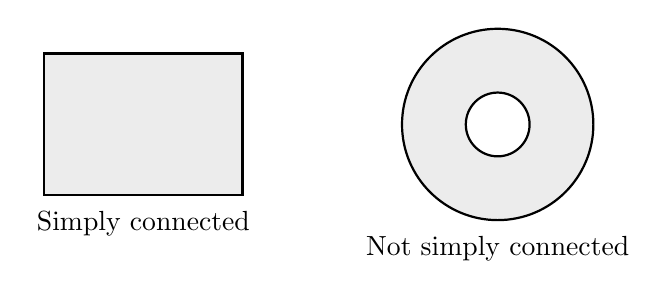
\begin{tikzpicture}[scale=0.9]
\begin{scope}[xshift=-2.5cm]
\fill[gray!15] (-1.4,-1) rectangle (1.4,1);
\draw[thick] (-1.4,-1) rectangle (1.4,1);
\node at (0,-1.4) {Simply connected};
\end{scope}

\begin{scope}[xshift=2.5cm]
\fill[gray!15,even odd rule] (0,0) circle (1.35) (0,0) circle (0.45);
\draw[thick] (0,0) circle (1.35);
\draw[thick] (0,0) circle (0.45);
\node at (0,-1.75) {Not simply connected};
\end{scope}
\end{tikzpicture}
\end{center}

The rigorous topological meaning is developed later in Topology.

%%%%%%%%%%%%%%%%%%%%%%%%%%%%%%%%%%%%%%%%%%%%%%%%%%%%%%%%%%%%
\subsection{Why Domain Conditions Matter}
\label{subsec:domain-conditions-conservative}
%%%%%%%%%%%%%%%%%%%%%%%%%%%%%%%%%%%%%%%%%%%%%%%%%%%%%%%%%%%%

Consider

\[ \vect{F}(x,y)
=
\left\langle
-\frac{y}{x^2+y^2},
\frac{x}{x^2+y^2}
\right\rangle. \]

Away from the origin,

\[ P_y=Q_x. \]

However, the field is not defined at

\[ (0,0). \]

The punctured plane

\[ \R^2\setminus\{(0,0)\} \]

has a hole.

The integral around the unit circle is nonzero:

\[ \oint_C\vect{F}\cdot d\vect{r}=2\pi. \]

Thus equality of cross-partials alone is not enough without appropriate
domain hypotheses.

%%%%%%%%%%%%%%%%%%%%%%%%%%%%%%%%%%%%%%%%%%%%%%%%%%%%%%%%%%%%
\subsection{The Del Operator}
\label{subsec:del-operator}
%%%%%%%%%%%%%%%%%%%%%%%%%%%%%%%%%%%%%%%%%%%%%%%%%%%%%%%%%%%%

In three dimensions, the symbolic differential operator

\[ \nabla
=
\left\langle
\frac{\partial}{\partial x},
\frac{\partial}{\partial y},
\frac{\partial}{\partial z}
\right\rangle \]

is called the \emph{del operator} or \emph{nabla operator}.

The symbol \(\nabla\) was introduced earlier for the gradient.

Its meaning depends on how it is combined with a scalar or vector field.

The three central combinations are

\[ \nabla f,\qquad \nabla\cdot\vect{F},\qquad \nabla\times\vect{F}. \]

These correspond to gradient, divergence, and curl.

%%%%%%%%%%%%%%%%%%%%%%%%%%%%%%%%%%%%%%%%%%%%%%%%%%%%%%%%%%%%
\subsection{Gradient, Divergence, and Curl}
\label{subsec:grad-div-curl}
%%%%%%%%%%%%%%%%%%%%%%%%%%%%%%%%%%%%%%%%%%%%%%%%%%%%%%%%%%%%

The three major differential operations may be summarized as

\[
\begin{array}{ccl}
\text{Gradient} &:& \text{scalar field}\longrightarrow\text{vector field},\\[1mm]
\text{Divergence} &:& \text{vector field}\longrightarrow\text{scalar field},\\[1mm]
\text{Curl} &:& \text{vector field}\longrightarrow\text{vector field}.
\end{array}
\]

In symbols,

\[ f\xrightarrow{\nabla}\nabla f, \qquad
\vect{F}\xrightarrow{\nabla\cdot}\nabla\cdot\vect{F}, \qquad
\vect{F}\xrightarrow{\nabla\times}\nabla\times\vect{F}. \]

%%%%%%%%%%%%%%%%%%%%%%%%%%%%%%%%%%%%%%%%%%%%%%%%%%%%%%%%%%%%
\subsection{Divergence}
\label{subsec:divergence}
%%%%%%%%%%%%%%%%%%%%%%%%%%%%%%%%%%%%%%%%%%%%%%%%%%%%%%%%%%%%

\begin{definitionbox}{Divergence}
For
\[ \vect{F}=\langle P,Q,R\rangle, \]
the divergence is
\[ \boxed{
\nabla\cdot\vect{F}
=
\frac{\partial P}{\partial x}
+
\frac{\partial Q}{\partial y}
+
\frac{\partial R}{\partial z}.
} \]
\end{definitionbox}

The notation

\[ \nabla\cdot\vect{F} \]

is read ``the divergence of \(\vect{F}\).''

It is also written

\[ \operatorname{div}\vect{F}. \]

%%%%%%%%%%%%%%%%%%%%%%%%%%%%%%%%%%%%%%%%%%%%%%%%%%%%%%%%%%%%
\subsection{Meaning of Divergence}
\label{subsec:meaning-divergence}
%%%%%%%%%%%%%%%%%%%%%%%%%%%%%%%%%%%%%%%%%%%%%%%%%%%%%%%%%%%%

Divergence measures the local tendency of a vector field to flow outward or
inward.

Informally:

\begin{itemize}
    \item \(\nabla\cdot\vect{F}>0\): source-like behavior;
    \item \(\nabla\cdot\vect{F}<0\): sink-like behavior;
    \item \(\nabla\cdot\vect{F}=0\): no net local expansion.
\end{itemize}

\begin{center}
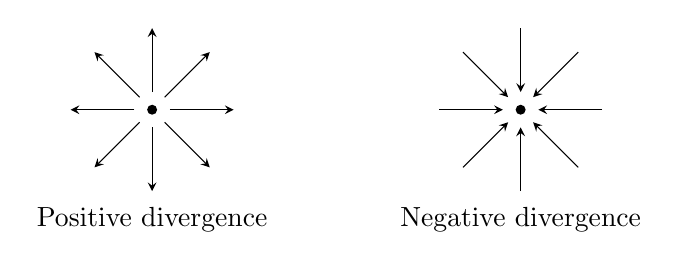
\begin{tikzpicture}[scale=0.9,>=stealth]
\begin{scope}[xshift=-2.6cm]
\fill (0,0) circle (2pt);
\foreach \a in {0,45,...,315}
    \draw[->] (\a:0.25)--(\a:1.15);
\node at (0,-1.55) {Positive divergence};
\end{scope}

\begin{scope}[xshift=2.6cm]
\fill (0,0) circle (2pt);
\foreach \a in {0,45,...,315}
    \draw[->] (\a:1.15)--(\a:0.25);
\node at (0,-1.55) {Negative divergence};
\end{scope}
\end{tikzpicture}
\end{center}

%%%%%%%%%%%%%%%%%%%%%%%%%%%%%%%%%%%%%%%%%%%%%%%%%%%%%%%%%%%%
\subsection{Worked Example: Divergence}
\label{subsec:worked-divergence}
%%%%%%%%%%%%%%%%%%%%%%%%%%%%%%%%%%%%%%%%%%%%%%%%%%%%%%%%%%%%

\begin{workedexamplebox}{Computing Divergence}

Let

\[ \vect{F}(x,y,z)=\langle x^2,xy,z^3\rangle. \]

Find \(\nabla\cdot\vect{F}\).

\begin{tabularx}{\textwidth}{@{}>{\raggedright\arraybackslash}p{0.42\textwidth}X@{}}
Differentiate the first component with respect to \(x\). &
\(P_x=2x\)\\
Differentiate the second component with respect to \(y\). &
\(Q_y=x\)\\
Differentiate the third component with respect to \(z\). &
\(R_z=3z^2\)\\
Add the results. &
\(2x+x+3z^2=3x+3z^2\)
\end{tabularx}

\begin{answerbox}
\[ \boxed{\nabla\cdot\vect{F}=3x+3z^2.} \]
\end{answerbox}
\end{workedexamplebox}

%%%%%%%%%%%%%%%%%%%%%%%%%%%%%%%%%%%%%%%%%%%%%%%%%%%%%%%%%%%%
\subsection{Divergence-Free Fields}
\label{subsec:divergence-free}
%%%%%%%%%%%%%%%%%%%%%%%%%%%%%%%%%%%%%%%%%%%%%%%%%%%%%%%%%%%%

A vector field satisfying

\[ \nabla\cdot\vect{F}=0 \]

is called \emph{divergence-free} or \emph{solenoidal}.

Such fields arise in incompressible fluid flow and magnetic-field models.

The equation

\[ \nabla\cdot\vect{F}=0 \]

does not mean the vector field itself is zero.

It means its local net outward flow vanishes.

%%%%%%%%%%%%%%%%%%%%%%%%%%%%%%%%%%%%%%%%%%%%%%%%%%%%%%%%%%%%
\subsection{Curl}
\label{subsec:curl}
%%%%%%%%%%%%%%%%%%%%%%%%%%%%%%%%%%%%%%%%%%%%%%%%%%%%%%%%%%%%

\begin{definitionbox}{Curl}
For
\[ \vect{F}=\langle P,Q,R\rangle, \]
the curl is
\[ \boxed{
\nabla\times\vect{F}
=
\left\langle
R_y-Q_z,\,
P_z-R_x,\,
Q_x-P_y
\right\rangle.
} \]
\end{definitionbox}

The notation

\[ \nabla\times\vect{F} \]

is read ``the curl of \(\vect{F}\).''

It is also written

\[ \operatorname{curl}\vect{F}. \]

%%%%%%%%%%%%%%%%%%%%%%%%%%%%%%%%%%%%%%%%%%%%%%%%%%%%%%%%%%%%
\subsection{Determinant Mnemonic for Curl}
\label{subsec:curl-determinant}
%%%%%%%%%%%%%%%%%%%%%%%%%%%%%%%%%%%%%%%%%%%%%%%%%%%%%%%%%%%%

A common mnemonic is

\[
\nabla\times\vect{F}
=
\begin{vmatrix}
\vect{i} & \vect{j} & \vect{k}\\
\dfrac{\partial}{\partial x} &
\dfrac{\partial}{\partial y} &
\dfrac{\partial}{\partial z}\\
P & Q & R
\end{vmatrix}.
\]

This determinant notation is symbolic rather than an ordinary determinant,
but it helps remember the component formula.

%%%%%%%%%%%%%%%%%%%%%%%%%%%%%%%%%%%%%%%%%%%%%%%%%%%%%%%%%%%%
\subsection{Meaning of Curl}
\label{subsec:meaning-curl}
%%%%%%%%%%%%%%%%%%%%%%%%%%%%%%%%%%%%%%%%%%%%%%%%%%%%%%%%%%%%

Curl measures local rotational tendency.

Imagine placing a tiny paddle wheel in a flowing fluid.

If the wheel tends to rotate, the flow has nonzero curl at that point.

\begin{center}
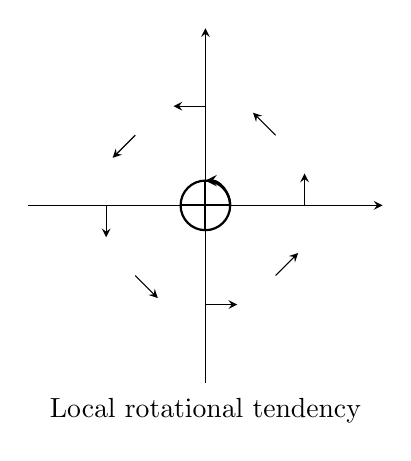
\begin{tikzpicture}[scale=0.9,>=stealth]
\draw[->] (-2.5,0)--(2.5,0);
\draw[->] (0,-2.5)--(0,2.5);
\foreach \a in {0,45,...,315}{
    \draw[->] (\a:1.4)--++({-0.45*sin(\a)},{0.45*cos(\a)});
}
\draw[thick] (0,0) circle (0.35);
\draw[thick] (-0.35,0)--(0.35,0);
\draw[thick] (0,-0.35)--(0,0.35);
\draw[->,thick] (0.35,0) arc[start angle=0,end angle=90,radius=0.35];
\node at (0,-2.9) {Local rotational tendency};
\end{tikzpicture}
\end{center}

%%%%%%%%%%%%%%%%%%%%%%%%%%%%%%%%%%%%%%%%%%%%%%%%%%%%%%%%%%%%
\subsection{Worked Example: Curl}
\label{subsec:worked-curl}
%%%%%%%%%%%%%%%%%%%%%%%%%%%%%%%%%%%%%%%%%%%%%%%%%%%%%%%%%%%%

\begin{workedexamplebox}{Computing Curl}

Let

\[ \vect{F}(x,y,z)=\langle-y,x,z\rangle. \]

Find \(\nabla\times\vect{F}\).

\begin{tabularx}{\textwidth}{@{}>{\raggedright\arraybackslash}p{0.42\textwidth}X@{}}
Identify the components. &
\(P=-y,\quad Q=x,\quad R=z\)\\
Compute the first component. &
\(R_y-Q_z=0-0=0\)\\
Compute the second component. &
\(P_z-R_x=0-0=0\)\\
Compute the third component. &
\(Q_x-P_y=1-(-1)=2\)
\end{tabularx}

\begin{answerbox}
\[ \boxed{\nabla\times\vect{F}=\langle0,0,2\rangle.} \]
\end{answerbox}
\end{workedexamplebox}

%%%%%%%%%%%%%%%%%%%%%%%%%%%%%%%%%%%%%%%%%%%%%%%%%%%%%%%%%%%%
\subsection{Irrotational Fields}
\label{subsec:irrotational-fields}
%%%%%%%%%%%%%%%%%%%%%%%%%%%%%%%%%%%%%%%%%%%%%%%%%%%%%%%%%%%%

A vector field satisfying

\[ \nabla\times\vect{F}=\vect{0} \]

is called \emph{irrotational}.

Every sufficiently smooth gradient field satisfies

\[ \boxed{\nabla\times(\nabla f)=\vect{0}.} \]

Thus conservative fields are locally curl-free.

On suitable simply connected domains, the converse also holds.

%%%%%%%%%%%%%%%%%%%%%%%%%%%%%%%%%%%%%%%%%%%%%%%%%%%%%%%%%%%%
\subsection{Divergence of a Curl}
\label{subsec:divergence-of-curl}
%%%%%%%%%%%%%%%%%%%%%%%%%%%%%%%%%%%%%%%%%%%%%%%%%%%%%%%%%%%%

For sufficiently smooth vector fields,

\[ \boxed{\nabla\cdot(\nabla\times\vect{F})=0.} \]

Thus every curl field is divergence-free.

Together with

\[ \nabla\times(\nabla f)=\vect{0}, \]

these identities reveal an important structural sequence:

\[ \text{scalar field}
\xrightarrow{\nabla}
\text{vector field}
\xrightarrow{\nabla\times}
\text{vector field}
\xrightarrow{\nabla\cdot}
\text{scalar field}. \]

The composition of consecutive operations vanishes.

%%%%%%%%%%%%%%%%%%%%%%%%%%%%%%%%%%%%%%%%%%%%%%%%%%%%%%%%%%%%
\subsection{The Laplacian}
\label{subsec:laplacian}
%%%%%%%%%%%%%%%%%%%%%%%%%%%%%%%%%%%%%%%%%%%%%%%%%%%%%%%%%%%%

Applying divergence to a gradient produces the \emph{Laplacian}.

\begin{definitionbox}{Laplacian}
For a scalar field \(f(x,y,z)\),
\[ \boxed{
\nabla^2f
=
f_{xx}+f_{yy}+f_{zz}.
} \]
\end{definitionbox}

The notation

\[ \nabla^2f \]

is read ``the Laplacian of \(f\).''

Another common notation is

\[ \Delta f. \]

Here the capital Greek letter \(\Delta\), called delta, represents the
Laplacian operator in this context.

%%%%%%%%%%%%%%%%%%%%%%%%%%%%%%%%%%%%%%%%%%%%%%%%%%%%%%%%%%%%
\subsection{Harmonic Functions}
\label{subsec:harmonic-functions-vector-calculus}
%%%%%%%%%%%%%%%%%%%%%%%%%%%%%%%%%%%%%%%%%%%%%%%%%%%%%%%%%%%%

A twice-differentiable function satisfying

\[ \nabla^2f=0 \]

is called \emph{harmonic}.

The equation

\[ \boxed{\nabla^2f=0} \]

is Laplace's equation.

Harmonic functions arise in:

\begin{itemize}
    \item steady-state heat flow;
    \item electrostatic potential;
    \item gravitational potential;
    \item fluid mechanics;
    \item complex analysis.
\end{itemize}

Their deeper theory belongs to Partial Differential Equations, Complex
Analysis, and Potential Theory.

%%%%%%%%%%%%%%%%%%%%%%%%%%%%%%%%%%%%%%%%%%%%%%%%%%%%%%%%%%%%
\subsection{Parameterized Surfaces}
\label{subsec:parameterized-surfaces}
%%%%%%%%%%%%%%%%%%%%%%%%%%%%%%%%%%%%%%%%%%%%%%%%%%%%%%%%%%%%

A surface in three-dimensional space can be described using two parameters.

A parameterized surface has the form

\[ \vect{r}(u,v)
=
\langle x(u,v),y(u,v),z(u,v)\rangle. \]

For example, a sphere of radius \(R\) can be parameterized by

\[ \vect{r}(\phi,\theta)
=
\langle
R\sin\phi\cos\theta,\,
R\sin\phi\sin\theta,\,
R\cos\phi
\rangle. \]

Two parameters are needed because a surface is locally two-dimensional.

%%%%%%%%%%%%%%%%%%%%%%%%%%%%%%%%%%%%%%%%%%%%%%%%%%%%%%%%%%%%
\subsection{Tangent Vectors to a Surface}
\label{subsec:surface-tangent-vectors}
%%%%%%%%%%%%%%%%%%%%%%%%%%%%%%%%%%%%%%%%%%%%%%%%%%%%%%%%%%%%

For

\[ \vect{r}(u,v), \]

differentiate with respect to each parameter:

\[ \vect{r}_u=\frac{\partial\vect{r}}{\partial u},
\qquad
\vect{r}_v=\frac{\partial\vect{r}}{\partial v}. \]

These vectors lie tangent to the surface.

At a regular point, they span the tangent plane.

\begin{center}
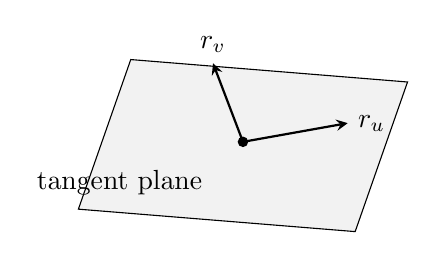
\begin{tikzpicture}[scale=0.95,>=stealth]
\draw[fill=gray!10] (-2,-0.8) -- (1.7,-1.1) -- (2.4,0.9) -- (-1.3,1.2) -- cycle;
\coordinate (P) at (0.2,0.1);
\fill (P) circle (2pt);
\draw[->,thick] (P)--++(1.4,0.25) node[right] {$\vect{r}_u$};
\draw[->,thick] (P)--++(-0.4,1.05) node[above] {$\vect{r}_v$};
\node at (-1.45,-0.45) {tangent plane};
\end{tikzpicture}
\end{center}

%%%%%%%%%%%%%%%%%%%%%%%%%%%%%%%%%%%%%%%%%%%%%%%%%%%%%%%%%%%%
\subsection{Normal Vectors to a Surface}
\label{subsec:surface-normal-vectors}
%%%%%%%%%%%%%%%%%%%%%%%%%%%%%%%%%%%%%%%%%%%%%%%%%%%%%%%%%%%%

A vector perpendicular to both tangent vectors is obtained using the cross
product:

\[ \vect{r}_u\times\vect{r}_v. \]

Therefore,

\[ \boxed{\vect{n}=\vect{r}_u\times\vect{r}_v} \]

is a normal vector whenever the cross product is nonzero.

A unit normal is

\[ \boxed{
\widehat{\vect{n}}
=
\frac{\vect{r}_u\times\vect{r}_v}
{\norm{\vect{r}_u\times\vect{r}_v}}.
} \]

%%%%%%%%%%%%%%%%%%%%%%%%%%%%%%%%%%%%%%%%%%%%%%%%%%%%%%%%%%%%
\subsection{Orientation of Surfaces}
\label{subsec:surface-orientation}
%%%%%%%%%%%%%%%%%%%%%%%%%%%%%%%%%%%%%%%%%%%%%%%%%%%%%%%%%%%%

An orientable surface admits a continuous choice of unit normal vector.

Choosing one of the two possible directions gives the surface an
\emph{orientation}.

For a closed surface, the standard positive orientation is the
\emph{outward} normal.

For an open surface, the problem usually specifies an orientation such as:

\begin{itemize}
    \item upward;
    \item downward;
    \item outward;
    \item inward.
\end{itemize}

%%%%%%%%%%%%%%%%%%%%%%%%%%%%%%%%%%%%%%%%%%%%%%%%%%%%%%%%%%%%
\subsection{Surface Area Element}
\label{subsec:surface-area-element}
%%%%%%%%%%%%%%%%%%%%%%%%%%%%%%%%%%%%%%%%%%%%%%%%%%%%%%%%%%%%

For a parameterized surface

\[ \vect{r}(u,v), \]

the surface-area element is

\[ \boxed{
dS
=
\norm{\vect{r}_u\times\vect{r}_v}\,du\,dv.
} \]

Thus the area of a surface \(S\) is

\[ \boxed{
\operatorname{Area}(S)
=
\iint_D
\norm{\vect{r}_u\times\vect{r}_v}\,du\,dv.
} \]

%%%%%%%%%%%%%%%%%%%%%%%%%%%%%%%%%%%%%%%%%%%%%%%%%%%%%%%%%%%%
\subsection{Scalar Surface Integrals}
\label{subsec:scalar-surface-integrals}
%%%%%%%%%%%%%%%%%%%%%%%%%%%%%%%%%%%%%%%%%%%%%%%%%%%%%%%%%%%%

If \(f\) is a scalar field defined on a surface \(S\), then

\[ \iint_Sf\,dS \]

is a scalar surface integral.

Using a parameterization,

\[ \boxed{
\iint_Sf\,dS
=
\iint_D
f(\vect{r}(u,v))
\norm{\vect{r}_u\times\vect{r}_v}\,du\,dv.
} \]

For example, if a thin shell has surface density \(\rho\), its mass is

\[ m=\iint_S\rho\,dS. \]

%%%%%%%%%%%%%%%%%%%%%%%%%%%%%%%%%%%%%%%%%%%%%%%%%%%%%%%%%%%%
\subsection{Graphs as Parameterized Surfaces}
\label{subsec:graphs-parameterized-surfaces}
%%%%%%%%%%%%%%%%%%%%%%%%%%%%%%%%%%%%%%%%%%%%%%%%%%%%%%%%%%%%

A graph

\[ z=g(x,y) \]

can be parameterized by

\[ \vect{r}(x,y)=\langle x,y,g(x,y)\rangle. \]

Then

\[ \vect{r}_x=\langle1,0,g_x\rangle,
\qquad
\vect{r}_y=\langle0,1,g_y\rangle. \]

Their cross product is

\[ \vect{r}_x\times\vect{r}_y
=
\langle-g_x,-g_y,1\rangle. \]

Hence

\[ \boxed{dS=\sqrt{1+g_x^2+g_y^2}\,dA.} \]

%%%%%%%%%%%%%%%%%%%%%%%%%%%%%%%%%%%%%%%%%%%%%%%%%%%%%%%%%%%%
\subsection{Flux}
\label{subsec:flux}
%%%%%%%%%%%%%%%%%%%%%%%%%%%%%%%%%%%%%%%%%%%%%%%%%%%%%%%%%%%%

Flux measures how much of a vector field passes through a surface.

If \(\widehat{\vect{n}}\) is the chosen unit normal, then the scalar quantity

\[ \vect{F}\cdot\widehat{\vect{n}} \]

measures the component of the field perpendicular to the surface.

The total flux is

\[ \boxed{
\iint_S\vect{F}\cdot\widehat{\vect{n}}\,dS.
} \]

%%%%%%%%%%%%%%%%%%%%%%%%%%%%%%%%%%%%%%%%%%%%%%%%%%%%%%%%%%%%
\subsection{Vector Surface Element}
\label{subsec:vector-surface-element}
%%%%%%%%%%%%%%%%%%%%%%%%%%%%%%%%%%%%%%%%%%%%%%%%%%%%%%%%%%%%

It is convenient to combine orientation and surface area into the vector
surface element

\[ d\vect{S}=\widehat{\vect{n}}\,dS. \]

Thus flux can be written compactly as

\[ \boxed{\iint_S\vect{F}\cdot d\vect{S}.} \]

For a parameterized surface with compatible orientation,

\[ d\vect{S}
=
(\vect{r}_u\times\vect{r}_v)\,du\,dv. \]

Therefore,

\[ \boxed{
\iint_S\vect{F}\cdot d\vect{S}
=
\iint_D
\vect{F}(\vect{r}(u,v))
\cdot
(\vect{r}_u\times\vect{r}_v)
\,du\,dv.
} \]

%%%%%%%%%%%%%%%%%%%%%%%%%%%%%%%%%%%%%%%%%%%%%%%%%%%%%%%%%%%%
\subsection{Worked Example: Flux Through a Plane}
\label{subsec:worked-flux-plane}
%%%%%%%%%%%%%%%%%%%%%%%%%%%%%%%%%%%%%%%%%%%%%%%%%%%%%%%%%%%%

\begin{workedexamplebox}{Flux Through a Horizontal Surface}

Let

\[ \vect{F}(x,y,z)=\langle x,y,z\rangle. \]

Find the upward flux through

\[ S:\ z=2,\qquad0\leq x\leq1,\quad0\leq y\leq1. \]

\begin{tabularx}{\textwidth}{@{}>{\raggedright\arraybackslash}p{0.42\textwidth}X@{}}
Choose the upward unit normal. &
\(\widehat{\vect{n}}=\langle0,0,1\rangle\)\\
Evaluate the field on \(z=2\). &
\(\vect{F}=\langle x,y,2\rangle\)\\
Take the dot product. &
\(\vect{F}\cdot\widehat{\vect{n}}=2\)\\
Construct the flux integral. &
\(\displaystyle \int_0^1\int_0^1 2\,dy\,dx\)\\
Evaluate. &
\(2\)
\end{tabularx}

\begin{answerbox}
\[ \boxed{\text{Flux}=2.} \]
\end{answerbox}
\end{workedexamplebox}

%%%%%%%%%%%%%%%%%%%%%%%%%%%%%%%%%%%%%%%%%%%%%%%%%%%%%%%%%%%%
\subsection{Positive Orientation in the Plane}
\label{subsec:positive-orientation-plane}
%%%%%%%%%%%%%%%%%%%%%%%%%%%%%%%%%%%%%%%%%%%%%%%%%%%%%%%%%%%%

For a simple closed curve in the plane, the standard positive orientation
is counterclockwise.

When traversing the boundary counterclockwise, the enclosed region remains
on the left.

\begin{center}
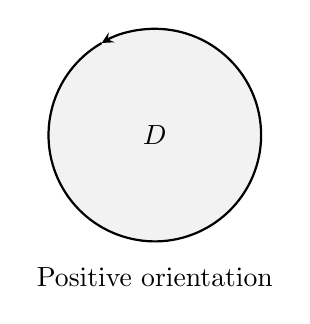
\begin{tikzpicture}[scale=0.9,>=stealth]
\fill[gray!10] (0,0) circle (1.5);
\draw[thick,->] (1.5,0) arc[start angle=0,end angle=120,radius=1.5];
\draw[thick] (120:1.5) arc[start angle=120,end angle=360,radius=1.5];
\node at (0,0) {$D$};
\node at (0,-2) {Positive orientation};
\end{tikzpicture}
\end{center}

This convention is essential in Green's Theorem.

%%%%%%%%%%%%%%%%%%%%%%%%%%%%%%%%%%%%%%%%%%%%%%%%%%%%%%%%%%%%
\subsection{Green's Theorem}
\label{subsec:greens-theorem}
%%%%%%%%%%%%%%%%%%%%%%%%%%%%%%%%%%%%%%%%%%%%%%%%%%%%%%%%%%%%

Green's Theorem connects a line integral around a closed planar curve with
a double integral over the enclosed region.

\begin{theorem}[Green's Theorem]
Let \(C\) be a positively oriented, piecewise smooth, simple closed curve
bounding a region \(D\). If \(P\) and \(Q\) have continuous partial
derivatives on an open region containing \(D\), then
\[ \boxed{
\oint_C P\,dx+Q\,dy
=
\iint_D
\left(
\frac{\partial Q}{\partial x}
-
\frac{\partial P}{\partial y}
\right)dA.
} \]
\end{theorem}

The quantity

\[ Q_x-P_y \]

is the two-dimensional scalar analogue of curl.

%%%%%%%%%%%%%%%%%%%%%%%%%%%%%%%%%%%%%%%%%%%%%%%%%%%%%%%%%%%%
\subsection{Meaning of Green's Theorem}
\label{subsec:meaning-greens-theorem}
%%%%%%%%%%%%%%%%%%%%%%%%%%%%%%%%%%%%%%%%%%%%%%%%%%%%%%%%%%%%

Green's Theorem says that total circulation around the boundary equals the
accumulated local rotation throughout the interior.

Symbolically,

\[ \boxed{\text{boundary circulation}
=
\text{interior curl accumulation}.} \]

\begin{center}
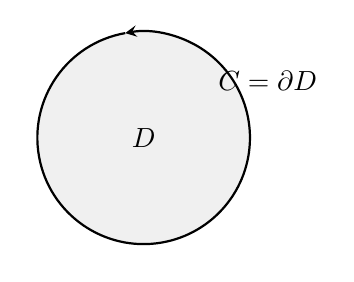
\begin{tikzpicture}[scale=0.9,>=stealth]
\fill[gray!12] (0,0) circle (1.5);
\draw[thick,->] (1.5,0) arc[start angle=0,end angle=100,radius=1.5];
\draw[thick] (100:1.5) arc[start angle=100,end angle=360,radius=1.5];
\node at (0,0) {$D$};
\node at (1.75,0.8) {$C=\partial D$};
\end{tikzpicture}
\end{center}

The notation

\[ \partial D \]

is read ``the boundary of \(D\).''

Here the symbol \(\partial\) denotes a boundary rather than a partial
derivative; the meaning is determined by context.

%%%%%%%%%%%%%%%%%%%%%%%%%%%%%%%%%%%%%%%%%%%%%%%%%%%%%%%%%%%%
\subsection{Worked Example: Green's Theorem}
\label{subsec:worked-greens-theorem}
%%%%%%%%%%%%%%%%%%%%%%%%%%%%%%%%%%%%%%%%%%%%%%%%%%%%%%%%%%%%

\begin{workedexamplebox}{Converting a Line Integral to an Area Integral}

Evaluate

\[ \oint_C -y\,dx+x\,dy, \]

where \(C\) is the positively oriented unit circle.

\begin{tabularx}{\textwidth}{@{}>{\raggedright\arraybackslash}p{0.42\textwidth}X@{}}
Identify \(P\) and \(Q\). &
\(P=-y,\quad Q=x\)\\
Compute \(Q_x\). &
\(Q_x=1\)\\
Compute \(P_y\). &
\(P_y=-1\)\\
Apply Green's Theorem. &
\(\displaystyle \iint_D(1-(-1))\,dA\)\\
Simplify. &
\(\displaystyle 2\iint_DdA\)\\
Use the area of the unit disk. &
\(2\pi\)
\end{tabularx}

\begin{answerbox}
\[ \boxed{\oint_C -y\,dx+x\,dy=2\pi.} \]
\end{answerbox}
\end{workedexamplebox}

%%%%%%%%%%%%%%%%%%%%%%%%%%%%%%%%%%%%%%%%%%%%%%%%%%%%%%%%%%%%
\subsection{Flux Form of Green's Theorem}
\label{subsec:greens-flux-form}
%%%%%%%%%%%%%%%%%%%%%%%%%%%%%%%%%%%%%%%%%%%%%%%%%%%%%%%%%%%%

For

\[ \vect{F}=\langle P,Q\rangle, \]

Green's Theorem also has a flux form:

\[ \boxed{
\oint_C\vect{F}\cdot\vect{n}\,ds
=
\iint_D
\left(P_x+Q_y\right)dA.
} \]

Since

\[ P_x+Q_y=\nabla\cdot\vect{F}, \]

this becomes

\[ \boxed{
\oint_C\vect{F}\cdot\vect{n}\,ds
=
\iint_D\nabla\cdot\vect{F}\,dA.
} \]

Thus outward boundary flux equals accumulated divergence in the region.

%%%%%%%%%%%%%%%%%%%%%%%%%%%%%%%%%%%%%%%%%%%%%%%%%%%%%%%%%%%%
\subsection{Green's Theorem and Area}
\label{subsec:greens-theorem-area}
%%%%%%%%%%%%%%%%%%%%%%%%%%%%%%%%%%%%%%%%%%%%%%%%%%%%%%%%%%%%

Green's Theorem can produce formulas for area.

Since

\[ \operatorname{Area}(D)=\iint_D1\,dA, \]

choose \(P,Q\) so that

\[ Q_x-P_y=1. \]

For example, choose

\[ P=0,\qquad Q=x. \]

Then

\[ \boxed{\operatorname{Area}(D)=\oint_Cx\,dy.} \]

Another symmetric formula is

\[ \boxed{
\operatorname{Area}(D)
=
\frac12\oint_C(x\,dy-y\,dx).
} \]

%%%%%%%%%%%%%%%%%%%%%%%%%%%%%%%%%%%%%%%%%%%%%%%%%%%%%%%%%%%%
\subsection{Boundary Orientation for Surfaces}
\label{subsec:boundary-orientation-surfaces}
%%%%%%%%%%%%%%%%%%%%%%%%%%%%%%%%%%%%%%%%%%%%%%%%%%%%%%%%%%%%

For an oriented surface \(S\), the boundary curve \(C=\partial S\) inherits
an orientation.

A common right-hand-rule interpretation is:

\begin{itemize}
    \item point the right thumb in the direction of the chosen surface normal;
    \item the curled fingers indicate the positive direction around the
    boundary.
\end{itemize}

For an upward-oriented horizontal surface, the positive boundary direction
is counterclockwise when viewed from above.

%%%%%%%%%%%%%%%%%%%%%%%%%%%%%%%%%%%%%%%%%%%%%%%%%%%%%%%%%%%%
\subsection{Stokes' Theorem}
\label{subsec:stokes-theorem}
%%%%%%%%%%%%%%%%%%%%%%%%%%%%%%%%%%%%%%%%%%%%%%%%%%%%%%%%%%%%

Stokes' Theorem generalizes Green's circulation theorem from planar regions
to oriented surfaces in three-dimensional space.

\begin{theorem}[Stokes' Theorem]
Let \(S\) be an oriented smooth surface with positively oriented boundary
curve \(C=\partial S\). Under suitable smoothness conditions on
\(\vect{F}\),
\[ \boxed{
\oint_C\vect{F}\cdot d\vect{r}
=
\iint_S
(\nabla\times\vect{F})\cdot\widehat{\vect{n}}\,dS.
} \]
\end{theorem}

Equivalently,

\[ \boxed{
\oint_{\partial S}\vect{F}\cdot d\vect{r}
=
\iint_S(\nabla\times\vect{F})\cdot d\vect{S}.
} \]

%%%%%%%%%%%%%%%%%%%%%%%%%%%%%%%%%%%%%%%%%%%%%%%%%%%%%%%%%%%%
\subsection{Meaning of Stokes' Theorem}
\label{subsec:meaning-stokes-theorem}
%%%%%%%%%%%%%%%%%%%%%%%%%%%%%%%%%%%%%%%%%%%%%%%%%%%%%%%%%%%%

Stokes' Theorem states that circulation around the boundary of a surface
equals the total normal component of curl through the surface.

Symbolically,

\[ \boxed{\text{boundary circulation}
=
\text{surface curl accumulation}.} \]

\begin{center}
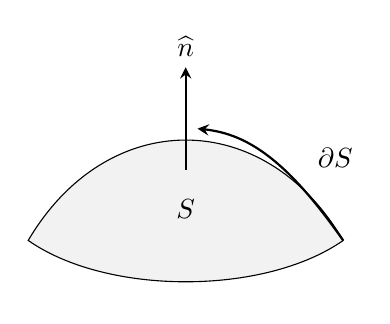
\begin{tikzpicture}[scale=1,>=stealth]
\draw[fill=gray!10]
(-2,-0.6) .. controls (-1,1.1) and (1,1.1) .. (2,-0.6)
.. controls (1,-1.3) and (-1,-1.3) .. cycle;

\draw[thick,->]
(2,-0.6) .. controls (1.3,0.4) and (0.8,0.75) .. (0.15,0.82);

\node at (0,-0.2) {$S$};
\node at (1.9,0.45) {$\partial S$};

\draw[->,thick] (0,0.3)--(0,1.6) node[above] {$\widehat{\vect{n}}$};
\end{tikzpicture}
\end{center}

%%%%%%%%%%%%%%%%%%%%%%%%%%%%%%%%%%%%%%%%%%%%%%%%%%%%%%%%%%%%
\subsection{Choosing a Surface in Stokes' Theorem}
\label{subsec:choosing-stokes-surface}
%%%%%%%%%%%%%%%%%%%%%%%%%%%%%%%%%%%%%%%%%%%%%%%%%%%%%%%%%%%%

Stokes' Theorem depends on the boundary curve, not on a unique spanning
surface.

If two appropriately oriented surfaces \(S_1\) and \(S_2\) share the same
boundary \(C\), then

\[ \iint_{S_1}(\nabla\times\vect{F})\cdot d\vect{S}
=
\iint_{S_2}(\nabla\times\vect{F})\cdot d\vect{S}. \]

Therefore, one should often choose the easiest surface having the required
boundary.

This can transform a difficult curved-surface integral into an easier planar
integral.

%%%%%%%%%%%%%%%%%%%%%%%%%%%%%%%%%%%%%%%%%%%%%%%%%%%%%%%%%%%%
\subsection{Worked Example: Stokes' Theorem}
\label{subsec:worked-stokes-theorem}
%%%%%%%%%%%%%%%%%%%%%%%%%%%%%%%%%%%%%%%%%%%%%%%%%%%%%%%%%%%%

\begin{workedexamplebox}{Circulation Around a Circle}

Let

\[ \vect{F}(x,y,z)=\langle-y,x,z\rangle. \]

Let \(C\) be the unit circle in the \(xy\)-plane oriented counterclockwise
when viewed from above. Evaluate

\[ \oint_C\vect{F}\cdot d\vect{r}. \]

\begin{tabularx}{\textwidth}{@{}>{\raggedright\arraybackslash}p{0.42\textwidth}X@{}}
Use the unit disk as \(S\). &
\(\widehat{\vect{n}}=\langle0,0,1\rangle\)\\
Compute the curl. &
\(\nabla\times\vect{F}=\langle0,0,2\rangle\)\\
Take the normal component. &
\((\nabla\times\vect{F})\cdot\widehat{\vect{n}}=2\)\\
Apply Stokes' Theorem. &
\(\displaystyle \iint_S2\,dA\)\\
Use the disk area. &
\(2\pi\)
\end{tabularx}

\begin{answerbox}
\[ \boxed{\oint_C\vect{F}\cdot d\vect{r}=2\pi.} \]
\end{answerbox}
\end{workedexamplebox}

%%%%%%%%%%%%%%%%%%%%%%%%%%%%%%%%%%%%%%%%%%%%%%%%%%%%%%%%%%%%
\subsection{Closed Surfaces}
\label{subsec:closed-surfaces}
%%%%%%%%%%%%%%%%%%%%%%%%%%%%%%%%%%%%%%%%%%%%%%%%%%%%%%%%%%%%

A \emph{closed surface} completely encloses a three-dimensional region and
has no boundary curve.

Examples include:

\begin{itemize}
    \item spheres;
    \item ellipsoids;
    \item closed cylinders;
    \item closed boxes.
\end{itemize}

The standard orientation of a closed surface is outward.

A closed surface is often denoted by

\[ \partial E, \]

the boundary of a solid region \(E\).

%%%%%%%%%%%%%%%%%%%%%%%%%%%%%%%%%%%%%%%%%%%%%%%%%%%%%%%%%%%%
\subsection{The Divergence Theorem}
\label{subsec:divergence-theorem}
%%%%%%%%%%%%%%%%%%%%%%%%%%%%%%%%%%%%%%%%%%%%%%%%%%%%%%%%%%%%

The Divergence Theorem converts outward flux across a closed surface into a
triple integral of divergence throughout the enclosed volume.

\begin{theorem}[Divergence Theorem]
Let \(E\) be a solid region with positively oriented boundary surface
\(S=\partial E\). Under suitable smoothness conditions,
\[ \boxed{
\iint_S\vect{F}\cdot\widehat{\vect{n}}\,dS
=
\iiint_E\nabla\cdot\vect{F}\,dV.
} \]
\end{theorem}

Equivalently,

\[ \boxed{
\iint_{\partial E}\vect{F}\cdot d\vect{S}
=
\iiint_E\nabla\cdot\vect{F}\,dV.
} \]

%%%%%%%%%%%%%%%%%%%%%%%%%%%%%%%%%%%%%%%%%%%%%%%%%%%%%%%%%%%%
\subsection{Meaning of the Divergence Theorem}
\label{subsec:meaning-divergence-theorem}
%%%%%%%%%%%%%%%%%%%%%%%%%%%%%%%%%%%%%%%%%%%%%%%%%%%%%%%%%%%%

The Divergence Theorem states that total outward flow through the boundary
equals total source strength throughout the interior.

Symbolically,

\[ \boxed{\text{outward boundary flux}
=
\text{interior divergence accumulation}.} \]

\begin{center}
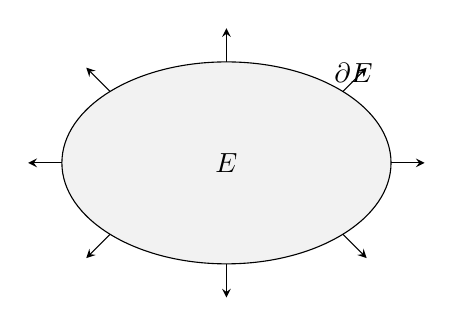
\begin{tikzpicture}[scale=0.95,>=stealth]
\draw[fill=gray!10] (0,0) ellipse (2.2 and 1.35);
\node at (0,0) {$E$};
\node at (1.7,1.2) {$\partial E$};

\foreach \a in {0,45,...,315}{
    \draw[->] ({2.2*cos(\a)},{1.35*sin(\a)})
    --++({0.45*cos(\a)},{0.45*sin(\a)});
}
\end{tikzpicture}
\end{center}

%%%%%%%%%%%%%%%%%%%%%%%%%%%%%%%%%%%%%%%%%%%%%%%%%%%%%%%%%%%%
\subsection{Worked Example: Divergence Theorem}
\label{subsec:worked-divergence-theorem}
%%%%%%%%%%%%%%%%%%%%%%%%%%%%%%%%%%%%%%%%%%%%%%%%%%%%%%%%%%%%

\begin{workedexamplebox}{Flux Through a Sphere}

Let

\[ \vect{F}(x,y,z)=\langle x,y,z\rangle. \]

Find the outward flux through the sphere

\[ x^2+y^2+z^2=R^2. \]

\begin{tabularx}{\textwidth}{@{}>{\raggedright\arraybackslash}p{0.42\textwidth}X@{}}
Compute the divergence. &
\(\nabla\cdot\vect{F}=1+1+1=3\)\\
Apply the Divergence Theorem. &
\(\displaystyle \iint_S\vect{F}\cdot d\vect{S}
=\iiint_E3\,dV\)\\
Use the volume of the sphere. &
\(\displaystyle 3\left(\frac43\pi R^3\right)\)\\
Simplify. &
\(4\pi R^3\)
\end{tabularx}

\begin{answerbox}
\[ \boxed{\text{Outward flux}=4\pi R^3.} \]
\end{answerbox}
\end{workedexamplebox}

%%%%%%%%%%%%%%%%%%%%%%%%%%%%%%%%%%%%%%%%%%%%%%%%%%%%%%%%%%%%
\subsection{Direct Flux versus the Divergence Theorem}
\label{subsec:direct-flux-vs-divergence}
%%%%%%%%%%%%%%%%%%%%%%%%%%%%%%%%%%%%%%%%%%%%%%%%%%%%%%%%%%%%

A closed-surface flux integral can often be evaluated in two ways.

\textbf{Direct method:}

\[ \iint_S\vect{F}\cdot\widehat{\vect{n}}\,dS. \]

\textbf{Divergence Theorem:}

\[ \iiint_E\nabla\cdot\vect{F}\,dV. \]

The better method depends on the geometry of the surface and the simplicity
of the divergence.

\begin{importantbox}
The major integral theorems are not merely theoretical identities. They are
also computational tools that allow a difficult integral to be replaced by
an easier equivalent integral.
\end{importantbox}

%%%%%%%%%%%%%%%%%%%%%%%%%%%%%%%%%%%%%%%%%%%%%%%%%%%%%%%%%%%%
\subsection{The Fundamental Theorem Pattern}
\label{subsec:fundamental-theorem-pattern}
%%%%%%%%%%%%%%%%%%%%%%%%%%%%%%%%%%%%%%%%%%%%%%%%%%%%%%%%%%%%

The major integral theorems share a common structure.

The Fundamental Theorem of Calculus says

\[ \int_{[a,b]}f'(x)\,dx=f(b)-f(a). \]

The Fundamental Theorem for Line Integrals says

\[ \int_C\nabla f\cdot d\vect{r}
=f(B)-f(A). \]

Green's Theorem says

\[ \oint_{\partial D}\vect{F}\cdot d\vect{r}
=
\iint_D\operatorname{curl}_{2D}\vect{F}\,dA. \]

Stokes' Theorem says

\[ \oint_{\partial S}\vect{F}\cdot d\vect{r}
=
\iint_S(\nabla\times\vect{F})\cdot d\vect{S}. \]

The Divergence Theorem says

\[ \iint_{\partial E}\vect{F}\cdot d\vect{S}
=
\iiint_E\nabla\cdot\vect{F}\,dV. \]

All of them connect an integral over a region to an integral over its
boundary.

%%%%%%%%%%%%%%%%%%%%%%%%%%%%%%%%%%%%%%%%%%%%%%%%%%%%%%%%%%%%
\subsection{Boundary of a Boundary}
\label{subsec:boundary-of-boundary}
%%%%%%%%%%%%%%%%%%%%%%%%%%%%%%%%%%%%%%%%%%%%%%%%%%%%%%%%%%%%

There is a deeper structural principle behind these theorems:

\[ \boxed{\partial(\partial\Omega)=0.} \]

This is read:

``the boundary of a boundary is zero.''

For example:

\begin{itemize}
    \item the boundary of an interval consists of endpoints;
    \item the boundary of a planar region is a closed curve;
    \item the boundary of a surface has endpoints only if the boundary curve
    itself is not closed;
    \item the boundary of a solid is a closed surface.
\end{itemize}

This idea later becomes central in topology, differential geometry, and
homology.

%%%%%%%%%%%%%%%%%%%%%%%%%%%%%%%%%%%%%%%%%%%%%%%%%%%%%%%%%%%%
\subsection{A Unified Stokes Viewpoint}
\label{subsec:generalized-stokes-preview}
%%%%%%%%%%%%%%%%%%%%%%%%%%%%%%%%%%%%%%%%%%%%%%%%%%%%%%%%%%%%

At a deeper level, the Fundamental Theorem of Calculus, Green's Theorem,
Stokes' Theorem, and the Divergence Theorem are manifestations of one
general principle:

\[ \boxed{\int_{\partial\Omega}\omega=\int_\Omega d\omega.} \]

The Greek letter

\[ \omega \]

is omega, pronounced ``oh-MAY-guh'' or ``oh-MEG-uh.''

Here \(\omega\) represents a differential form.

The symbol

\[ d\omega \]

represents its exterior derivative.

This formula is the generalized Stokes theorem.

Differential forms and exterior derivatives belong canonically to
Differential Geometry, so only the unifying idea is introduced here.

%%%%%%%%%%%%%%%%%%%%%%%%%%%%%%%%%%%%%%%%%%%%%%%%%%%%%%%%%%%%
\subsection{Comparison of the Major Integral Theorems}
\label{subsec:integral-theorem-comparison}
%%%%%%%%%%%%%%%%%%%%%%%%%%%%%%%%%%%%%%%%%%%%%%%%%%%%%%%%%%%%

\begin{center}
\begin{tabularx}{\textwidth}{@{}lXXX@{}}
\toprule
\textbf{Theorem} &
\textbf{Interior} &
\textbf{Boundary} &
\textbf{Differential Quantity}\\
\midrule
FTC &
Interval &
Endpoints &
Derivative\\
Line Integral FTC &
Curve &
Endpoints &
Gradient\\
Green &
Planar region &
Closed curve &
2D curl or divergence\\
Stokes &
Surface &
Closed curve &
Curl\\
Divergence &
Solid &
Closed surface &
Divergence\\
\bottomrule
\end{tabularx}
\end{center}

%%%%%%%%%%%%%%%%%%%%%%%%%%%%%%%%%%%%%%%%%%%%%%%%%%%%%%%%%%%%
\subsection{Circulation}
\label{subsec:circulation}
%%%%%%%%%%%%%%%%%%%%%%%%%%%%%%%%%%%%%%%%%%%%%%%%%%%%%%%%%%%%

For a closed curve \(C\), the circulation of a vector field is

\[ \boxed{\oint_C\vect{F}\cdot d\vect{r}.} \]

Circulation measures the tendency of the field to move along the curve.

Green's Theorem and Stokes' Theorem connect circulation to curl.

Thus:

\[ \boxed{\text{curl is the local source of circulation}.} \]

%%%%%%%%%%%%%%%%%%%%%%%%%%%%%%%%%%%%%%%%%%%%%%%%%%%%%%%%%%%%
\subsection{Flux and Divergence}
\label{subsec:flux-and-divergence}
%%%%%%%%%%%%%%%%%%%%%%%%%%%%%%%%%%%%%%%%%%%%%%%%%%%%%%%%%%%%

For a closed surface \(S\), outward flux is

\[ \boxed{\iint_S\vect{F}\cdot d\vect{S}.} \]

The Divergence Theorem connects this global flux to local divergence.

Thus:

\[ \boxed{\text{divergence is the local source of net outward flux}.} \]

This local-to-global relationship is one of the central themes of vector
calculus.

%%%%%%%%%%%%%%%%%%%%%%%%%%%%%%%%%%%%%%%%%%%%%%%%%%%%%%%%%%%%
\subsection{Conservative Fields and Energy}
\label{subsec:conservative-fields-energy}
%%%%%%%%%%%%%%%%%%%%%%%%%%%%%%%%%%%%%%%%%%%%%%%%%%%%%%%%%%%%

In mechanics, a conservative force field is often written

\[ \vect{F}=-\nabla U, \]

where \(U\) is potential energy.

Then the work from \(A\) to \(B\) is

\[ W=\int_C\vect{F}\cdot d\vect{r}. \]

Using the Fundamental Theorem for Line Integrals,

\[ W=-[U(B)-U(A)]. \]

Therefore,

\[ \boxed{W=U(A)-U(B).} \]

This explains why conservative forces permit potential-energy descriptions.

%%%%%%%%%%%%%%%%%%%%%%%%%%%%%%%%%%%%%%%%%%%%%%%%%%%%%%%%%%%%
\subsection{Vector Calculus in Fluid Flow}
\label{subsec:vector-calculus-fluid-flow}
%%%%%%%%%%%%%%%%%%%%%%%%%%%%%%%%%%%%%%%%%%%%%%%%%%%%%%%%%%%%

Suppose

\[ \vect{v}(x,y,z,t) \]

represents fluid velocity.

Then:

\begin{itemize}
    \item \(\vect{v}\) describes local direction and speed;
    \item \(\nabla\cdot\vect{v}\) measures local expansion or compression;
    \item \(\nabla\times\vect{v}\) measures local rotational tendency;
    \item flux integrals measure flow through surfaces;
    \item circulation integrals measure flow around curves.
\end{itemize}

For incompressible flow,

\[ \nabla\cdot\vect{v}=0. \]

%%%%%%%%%%%%%%%%%%%%%%%%%%%%%%%%%%%%%%%%%%%%%%%%%%%%%%%%%%%%
\subsection{Vector Calculus in Electromagnetism}
\label{subsec:vector-calculus-electromagnetism}
%%%%%%%%%%%%%%%%%%%%%%%%%%%%%%%%%%%%%%%%%%%%%%%%%%%%%%%%%%%%

Electric and magnetic fields are naturally modeled as vector fields.

Maxwell's equations use divergence and curl to describe how electric and
magnetic fields behave.

In differential form, the structure includes equations of the type

\[ \nabla\cdot\vect{E}=\text{source density}, \]

and

\[ \nabla\times\vect{E}
=\text{time-dependent magnetic effect}. \]

Their precise physical formulation belongs to Mathematical Physics.

The key mathematical point is that divergence and curl encode local field
behavior, while the integral theorems convert those local equations into
global statements.

%%%%%%%%%%%%%%%%%%%%%%%%%%%%%%%%%%%%%%%%%%%%%%%%%%%%%%%%%%%%
\subsection{Vector Calculus in Transport}
\label{subsec:vector-calculus-transport}
%%%%%%%%%%%%%%%%%%%%%%%%%%%%%%%%%%%%%%%%%%%%%%%%%%%%%%%%%%%%

Suppose a substance has concentration

\[ c(x,y,z,t) \]

and moves through a velocity field \(\vect{v}\).

The vector

\[ c\vect{v} \]

can represent transport flux.

The divergence

\[ \nabla\cdot(c\vect{v}) \]

then measures the net local rate at which transported material leaves a
small region.

Such ideas lead naturally to conservation laws and partial differential
equations.

%%%%%%%%%%%%%%%%%%%%%%%%%%%%%%%%%%%%%%%%%%%%%%%%%%%%%%%%%%%%
\subsection{Conservation Laws}
\label{subsec:conservation-laws-vector-calculus}
%%%%%%%%%%%%%%%%%%%%%%%%%%%%%%%%%%%%%%%%%%%%%%%%%%%%%%%%%%%%

Suppose \(\rho\) represents the density of some conserved quantity and
\(\vect{J}\) represents its flux.

A fundamental conservation equation is

\[ \boxed{\frac{\partial\rho}{\partial t}
+\nabla\cdot\vect{J}=0.} \]

This is called a \emph{continuity equation}.

It expresses the principle:

\[ \text{local accumulation}
+
\text{net outward flow}
=0. \]

Integrating over a region and applying the Divergence Theorem converts this
local equation into a global conservation law.

%%%%%%%%%%%%%%%%%%%%%%%%%%%%%%%%%%%%%%%%%%%%%%%%%%%%%%%%%%%%
\subsection{Integral and Differential Viewpoints}
\label{subsec:integral-differential-viewpoints}
%%%%%%%%%%%%%%%%%%%%%%%%%%%%%%%%%%%%%%%%%%%%%%%%%%%%%%%%%%%%

Vector calculus repeatedly connects two viewpoints.

\textbf{Differential viewpoint:}

Study what happens locally using

\[ \nabla f,\qquad
\nabla\cdot\vect{F},\qquad
\nabla\times\vect{F}. \]

\textbf{Integral viewpoint:}

Study accumulated behavior using

\[ \int_C,\qquad \iint_S,\qquad \iiint_E. \]

The major integral theorems provide bridges between these viewpoints.

\begin{conceptbox}
Vector calculus is fundamentally a theory connecting local differential
behavior to global integral behavior.
\end{conceptbox}

%%%%%%%%%%%%%%%%%%%%%%%%%%%%%%%%%%%%%%%%%%%%%%%%%%%%%%%%%%%%
\subsection{Common Errors}
\label{subsec:vector-calculus-common-errors}
%%%%%%%%%%%%%%%%%%%%%%%%%%%%%%%%%%%%%%%%%%%%%%%%%%%%%%%%%%%%

\subsubsection{Confusing Scalar and Vector Fields}

A scalar field returns a number:

\[ f:\R^n\to\R. \]

A vector field returns a vector:

\[ \vect{F}:\R^n\to\R^m. \]

%%%%%%%%%%%%%%%%%%%%%%%%%%%%%%%%%%%%%%%%%%%%%%%%%%%%%%%%%%%%
\subsubsection{Confusing Gradient, Divergence, and Curl}

Remember the input-output pattern:

\[ \text{scalar}\xrightarrow{\nabla}\text{vector}, \]

\[ \text{vector}\xrightarrow{\nabla\cdot}\text{scalar}, \]

\[ \text{vector}\xrightarrow{\nabla\times}\text{vector}. \]

%%%%%%%%%%%%%%%%%%%%%%%%%%%%%%%%%%%%%%%%%%%%%%%%%%%%%%%%%%%%
\subsubsection{Forgetting to Parameterize the Curve}

A line integral cannot usually be evaluated by substituting endpoints.

One must parameterize the curve unless a theorem such as the Fundamental
Theorem for Line Integrals eliminates the need.

%%%%%%%%%%%%%%%%%%%%%%%%%%%%%%%%%%%%%%%%%%%%%%%%%%%%%%%%%%%%
\subsubsection{Forgetting the Speed Factor in Scalar Line Integrals}

For

\[ \int_Cf\,ds, \]

the parameterized form contains

\[ \norm{\vect{r}'(t)}. \]

Thus

\[ \int_Cf\,ds
=
\int_a^bf(\vect{r}(t))
\norm{\vect{r}'(t)}\,dt. \]

%%%%%%%%%%%%%%%%%%%%%%%%%%%%%%%%%%%%%%%%%%%%%%%%%%%%%%%%%%%%
\subsubsection{Adding a Speed Factor to a Work Integral}

For

\[ \int_C\vect{F}\cdot d\vect{r}, \]

use

\[ \vect{F}(\vect{r}(t))\cdot\vect{r}'(t)\,dt. \]

Do not multiply by an additional

\[ \norm{\vect{r}'(t)}. \]

%%%%%%%%%%%%%%%%%%%%%%%%%%%%%%%%%%%%%%%%%%%%%%%%%%%%%%%%%%%%
\subsubsection{Ignoring Orientation}

Changing orientation reverses the sign of oriented line and flux integrals.

Always identify the required direction before calculating.

%%%%%%%%%%%%%%%%%%%%%%%%%%%%%%%%%%%%%%%%%%%%%%%%%%%%%%%%%%%%
\subsubsection{Assuming Zero Curl Always Means Conservative}

The domain matters.

A curl-free field may fail to be globally conservative on a region with
holes.

%%%%%%%%%%%%%%%%%%%%%%%%%%%%%%%%%%%%%%%%%%%%%%%%%%%%%%%%%%%%
\subsubsection{Assuming Zero Divergence Means Zero Field}

A field can be nonzero everywhere while satisfying

\[ \nabla\cdot\vect{F}=0. \]

Zero divergence describes local net flow, not vector magnitude.

%%%%%%%%%%%%%%%%%%%%%%%%%%%%%%%%%%%%%%%%%%%%%%%%%%%%%%%%%%%%
\subsubsection{Using the Wrong Normal}

Flux depends on orientation.

For closed surfaces, ``outward'' and ``inward'' produce opposite signs.

%%%%%%%%%%%%%%%%%%%%%%%%%%%%%%%%%%%%%%%%%%%%%%%%%%%%%%%%%%%%
\subsubsection{Forgetting the Surface-Area Factor}

For a parameterized surface,

\[ dS=\norm{\vect{r}_u\times\vect{r}_v}\,du\,dv. \]

The parameter-domain area element \(du\,dv\) is not generally the same as
surface area.

%%%%%%%%%%%%%%%%%%%%%%%%%%%%%%%%%%%%%%%%%%%%%%%%%%%%%%%%%%%%
\subsubsection{Using Green's Theorem on an Open Curve}

Green's Theorem requires a closed boundary curve.

%%%%%%%%%%%%%%%%%%%%%%%%%%%%%%%%%%%%%%%%%%%%%%%%%%%%%%%%%%%%
\subsubsection{Using the Divergence Theorem on an Open Surface}

The Divergence Theorem applies directly to closed surfaces.

An open surface must usually be closed by adding missing pieces.

%%%%%%%%%%%%%%%%%%%%%%%%%%%%%%%%%%%%%%%%%%%%%%%%%%%%%%%%%%%%
\subsubsection{Mismatching Stokes Orientation}

The orientation of the boundary curve must agree with the chosen surface
normal according to the right-hand rule.

%%%%%%%%%%%%%%%%%%%%%%%%%%%%%%%%%%%%%%%%%%%%%%%%%%%%%%%%%%%%
\subsubsection{Computing Directly When a Theorem Is Easier}

Before evaluating a difficult line or surface integral, check whether Green's
Theorem, Stokes' Theorem, the Divergence Theorem, or the Fundamental Theorem
for Line Integrals converts it into a simpler problem.

%%%%%%%%%%%%%%%%%%%%%%%%%%%%%%%%%%%%%%%%%%%%%%%%%%%%%%%%%%%%
\subsection{Exercises}
\label{subsec:vector-calculus-exercises}
%%%%%%%%%%%%%%%%%%%%%%%%%%%%%%%%%%%%%%%%%%%%%%%%%%%%%%%%%%%%

\begin{exercise}[1]
Classify each as a scalar field or vector field:
\[ T(x,y,z)=x^2+y^2+z^2,\qquad
\vect{F}(x,y)=\langle y,-x\rangle. \]
\end{exercise}

\begin{exercise}[1]
Evaluate
\[ \vect{F}(2,-1) \]
for
\[ \vect{F}(x,y)=\langle x+y,x-y\rangle. \]
\end{exercise}

\begin{exercise}[2]
Sketch several vectors from the field
\[ \vect{F}(x,y)=\langle x,y\rangle. \]
Describe the overall behavior.
\end{exercise}

\begin{exercise}[2]
Sketch several vectors from
\[ \vect{F}(x,y)=\langle-y,x\rangle. \]
Describe the overall behavior.
\end{exercise}

\begin{exercise}[1]
For
\[ \vect{r}(t)=\langle t,t^2,t^3\rangle, \]
find velocity and acceleration.
\end{exercise}

\begin{exercise}[2]
Find the length of
\[ \vect{r}(t)=\langle3t,4t\rangle,\qquad0\leq t\leq2. \]
\end{exercise}

\begin{exercise}[2]
Evaluate
\[ \int_Cx\,ds \]
where \(C\) is the line segment from \((0,0)\) to \((2,2)\).
\end{exercise}

\begin{exercise}[2]
A wire follows
\[ \vect{r}(t)=\langle t,t^2\rangle,\qquad0\leq t\leq1, \]
and has density
\[ \rho(x,y)=1+x. \]
Find its mass.
\end{exercise}

\begin{exercise}[2]
Evaluate
\[ \int_C\vect{F}\cdot d\vect{r} \]
for
\[ \vect{F}(x,y)=\langle x,y\rangle \]
along
\[ \vect{r}(t)=\langle t,t^2\rangle,\qquad0\leq t\leq1. \]
\end{exercise}

\begin{exercise}[2]
Evaluate
\[ \int_C y\,dx+x\,dy \]
along the line segment from \((0,0)\) to \((2,3)\).
\end{exercise}

\begin{exercise}[1]
Determine whether
\[ \vect{F}(x,y)=\langle2x,2y\rangle \]
is conservative and find a potential function.
\end{exercise}

\begin{exercise}[2]
Find a potential function for
\[ \vect{F}(x,y)=\langle2xy+y,\ x^2+x+3y^2\rangle. \]
\end{exercise}

\begin{exercise}[2]
Determine whether
\[ \vect{F}(x,y)=\langle y^2,2xy\rangle \]
is conservative.
\end{exercise}

\begin{exercise}[2]
Use the Fundamental Theorem for Line Integrals to evaluate
\[ \int_C\nabla f\cdot d\vect{r} \]
for
\[ f(x,y)=x^2+y^2 \]
from \((1,0)\) to \((3,4)\).
\end{exercise}

\begin{exercise}[2]
Suppose
\[ \vect{F}=\nabla f. \]
Explain why
\[ \oint_C\vect{F}\cdot d\vect{r}=0 \]
for every closed curve \(C\) in the domain.
\end{exercise}

\begin{exercise}[2]
Compute the divergence of
\[ \vect{F}(x,y,z)=\langle xy,yz,zx\rangle. \]
\end{exercise}

\begin{exercise}[2]
Compute the curl of
\[ \vect{F}(x,y,z)=\langle yz,xz,xy\rangle. \]
\end{exercise}

\begin{exercise}[2]
Determine whether
\[ \vect{F}(x,y,z)=\langle2x,2y,2z\rangle \]
is divergence-free or curl-free.
\end{exercise}

\begin{exercise}[2]
Verify directly that
\[ \nabla\times(\nabla f)=\vect{0} \]
for
\[ f(x,y,z)=x^2y+yz^2. \]
\end{exercise}

\begin{exercise}[2]
Verify directly that
\[ \nabla\cdot(\nabla\times\vect{F})=0 \]
for
\[ \vect{F}(x,y,z)=\langle xy,yz,zx\rangle. \]
\end{exercise}

\begin{exercise}[1]
Find the Laplacian of
\[ f(x,y,z)=x^2+y^2+z^2. \]
\end{exercise}

\begin{exercise}[2]
Determine whether
\[ f(x,y)=x^2-y^2 \]
is harmonic.
\end{exercise}

\begin{exercise}[2]
For
\[ \vect{r}(u,v)=\langle u,v,u^2+v^2\rangle, \]
find
\[ \vect{r}_u,\qquad\vect{r}_v,\qquad
\vect{r}_u\times\vect{r}_v. \]
\end{exercise}

\begin{exercise}[2]
Find a normal vector to
\[ z=x^2+y^2 \]
at \((1,1,2)\).
\end{exercise}

\begin{exercise}[2]
Find the surface area of
\[ z=0,\qquad0\leq x\leq2,\quad0\leq y\leq3 \]
using a surface integral.
\end{exercise}

\begin{exercise}[2]
Set up the surface-area integral for
\[ z=x^2+y^2 \]
above the unit disk.
\end{exercise}

\begin{exercise}[2]
Compute the upward flux of
\[ \vect{F}(x,y,z)=\langle0,0,z\rangle \]
through the plane
\[ z=3,\qquad0\leq x\leq2,\quad0\leq y\leq1. \]
\end{exercise}

\begin{exercise}[2]
Use Green's Theorem to evaluate
\[ \oint_C -y\,dx+x\,dy \]
where \(C\) is the positively oriented circle
\[ x^2+y^2=4. \]
\end{exercise}

\begin{exercise}[2]
Use Green's Theorem to evaluate
\[ \oint_C x^2\,dx+xy\,dy \]
where \(C\) is the positively oriented boundary of the unit square.
\end{exercise}

\begin{exercise}[2]
Use Green's Theorem to derive
\[ \operatorname{Area}(D)=\oint_Cx\,dy. \]
\end{exercise}

\begin{exercise}[3]
Use
\[ \operatorname{Area}(D)
=
\frac12\oint_C(x\,dy-y\,dx) \]
to calculate the area enclosed by the ellipse
\[ x=a\cos t,\qquad y=b\sin t,\qquad0\leq t\leq2\pi. \]
\end{exercise}

\begin{exercise}[2]
Use Stokes' Theorem to evaluate the circulation of
\[ \vect{F}(x,y,z)=\langle-y,x,0\rangle \]
around the unit circle in the \(xy\)-plane oriented counterclockwise from
above.
\end{exercise}

\begin{exercise}[2]
Suppose two oriented surfaces share the same positively oriented boundary
curve. Explain why Stokes' Theorem allows the curl flux through one surface
to be replaced by the curl flux through the other.
\end{exercise}

\begin{exercise}[2]
Use the Divergence Theorem to find the outward flux of
\[ \vect{F}(x,y,z)=\langle x,y,z\rangle \]
through the unit sphere.
\end{exercise}

\begin{exercise}[2]
Use the Divergence Theorem to calculate the outward flux of
\[ \vect{F}(x,y,z)=\langle x^3,y^3,z^3\rangle \]
through the boundary of the cube
\[ -1\leq x,y,z\leq1. \]
\end{exercise}

\begin{exercise}[3]
Let
\[ \vect{F}(x,y,z)=\langle x^2,y^2,z^2\rangle. \]
Compare direct flux integration with the Divergence Theorem for a rectangular
box.
\end{exercise}

\begin{exercise}[3]
A fluid has velocity field
\[ \vect{v}(x,y,z)=\langle x,-y,0\rangle. \]
Compute its divergence and interpret the result.
\end{exercise}

\begin{exercise}[3]
A fluid has velocity field
\[ \vect{v}(x,y,z)=\langle-y,x,0\rangle. \]
Compute its curl and interpret the result.
\end{exercise}

\begin{exercise}[3]
Show that if
\[ \vect{F}=\nabla f \]
and \(f\) has continuous second partial derivatives, then
\[ \nabla\times\vect{F}=\vect{0}. \]
\end{exercise}

\begin{exercise}[3]
Explain why
\[ \nabla\cdot(\nabla\times\vect{F})=0 \]
suggests that a field represented globally as a curl must be divergence-free.
\end{exercise}

\begin{exercise}[3]
Explain the common structural form of the Fundamental Theorem of Calculus,
Green's Theorem, Stokes' Theorem, and the Divergence Theorem.
\end{exercise}

%%%%%%%%%%%%%%%%%%%%%%%%%%%%%%%%%%%%%%%%%%%%%%%%%%%%%%%%%%%%
\subsection{Conceptual Summary}
\label{subsec:vector-calculus-summary}
%%%%%%%%%%%%%%%%%%%%%%%%%%%%%%%%%%%%%%%%%%%%%%%%%%%%%%%%%%%%

Vector calculus studies vector fields and their interaction with curves,
surfaces, and regions.

A vector field has the form

\[ \vect{F}=\langle P,Q,R\rangle. \]

Line integrals measure accumulation along curves:

\[ \int_Cf\,ds \]

for scalar fields and

\[ \int_C\vect{F}\cdot d\vect{r} \]

for vector fields.

If

\[ \vect{F}=\nabla f, \]

then the field is conservative and

\[ \int_C\vect{F}\cdot d\vect{r}=f(B)-f(A). \]

The central differential operators are

\[ \boxed{
\nabla f,\qquad
\nabla\cdot\vect{F},\qquad
\nabla\times\vect{F}.
} \]

Gradient measures directional change.

Divergence measures local source or sink behavior.

Curl measures local rotation.

Surface integrals accumulate quantities across surfaces:

\[ \iint_Sf\,dS. \]

Flux measures the normal passage of a vector field:

\[ \iint_S\vect{F}\cdot d\vect{S}. \]

The major integral theorems connect boundary behavior to interior behavior:

\[ \boxed{
\text{Green}
\quad
\text{Stokes}
\quad
\text{Divergence}.
} \]

Their common principle is that local differential information, accumulated
throughout a region, determines global behavior on its boundary.

\begin{center}
\begin{tikzpicture}[
    node distance=12mm and 15mm,
    box/.style={draw,rounded corners,align=center,inner sep=6pt},
    >=stealth
]
\node[box] (scalar) {Scalar field\\\(f\)};
\node[box,right=of scalar] (vector) {Vector field\\\(\vect{F}\)};
\node[box,below=of scalar] (grad) {Gradient\\\(\nabla f\)};
\node[box,below left=of vector] (div) {Divergence\\\(\nabla\cdot\vect{F}\)};
\node[box,below right=of vector] (curl) {Curl\\\(\nabla\times\vect{F}\)};
\node[box,below=22mm of vector] (theorems) {Integral Theorems\\Green, Stokes, Divergence};

\draw[->] (scalar)--(grad);
\draw[->] (vector)--(div);
\draw[->] (vector)--(curl);
\draw[->] (grad)--(theorems);
\draw[->] (div)--(theorems);
\draw[->] (curl)--(theorems);
\end{tikzpicture}
\end{center}

%%%%%%%%%%%%%%%%%%%%%%%%%%%%%%%%%%%%%%%%%%%%%%%%%%%%%%%%%%%%
\subsection{Section Connections}
\label{subsec:vector-calculus-connections}
%%%%%%%%%%%%%%%%%%%%%%%%%%%%%%%%%%%%%%%%%%%%%%%%%%%%%%%%%%%%

\chapterconnection{
Vector calculus extends multivariable calculus from scalar functions to
vector fields and develops the mathematics of circulation, flux, local
rotation, and local expansion. Line integrals generalize ordinary
integration to curves, while surface integrals generalize integration to
two-dimensional surfaces embedded in space. Conservative fields connect
gradients with path-independent work through the Fundamental Theorem for
Line Integrals. Divergence and curl describe local behavior of vector fields,
while Green's Theorem, Stokes' Theorem, and the Divergence Theorem convert
that local information into global boundary statements. These ideas form a
central foundation for differential geometry, partial differential
equations, fluid dynamics, electromagnetism, continuum mechanics,
conservation laws, mathematical physics, and geometric analysis.
}

%%%%%%%%%%%%%%%%%%%%%%%%%%%%%%%%%%%%%%%%%%%%%%%%%%%%%%%%%%%%
% SECTION SOURCE TRACKING
%%%%%%%%%%%%%%%%%%%%%%%%%%%%%%%%%%%%%%%%%%%%%%%%%%%%%%%%%%%%

%------------------------------------------------------------
% 5.4 Vector Calculus
%------------------------------------------------------------
%
% Sources:
%   - This section uses standard undergraduate vector-calculus theory
%     together with the multivariable calculus and linear algebra
%     foundations established earlier in the text.
%
% Used for:
%   - scalar and vector fields;
%   - parameterized curves;
%   - scalar line integrals;
%   - vector line integrals and work;
%   - conservative vector fields and potential functions;
%   - path independence;
%   - Fundamental Theorem for Line Integrals;
%   - gradient, divergence, curl, and Laplacian;
%   - parameterized surfaces and normal vectors;
%   - scalar surface integrals;
%   - flux integrals;
%   - Green's Theorem;
%   - Stokes' Theorem;
%   - Divergence Theorem;
%   - conservation-law interpretations;
%   - generalized Stokes theorem preview.
%
% Notes:
%   - Multivariable differentiation, gradients, multiple integrals,
%     coordinate transformations, and Jacobians are taught canonically in
%     Multivariable Calculus.
%   - Vector-space and linear-transformation theory is taught canonically in
%     Linear Algebra.
%   - Rigorous topological notions such as simple connectivity belong
%     canonically to Topology.
%   - Differential forms, exterior derivatives, tangent spaces, manifolds,
%     and the generalized Stokes theorem belong canonically to Differential
%     Geometry.
%   - Conservation laws and field equations are developed further in
%     Differential Equations and Mathematical Physics.
%   - Laplace's equation and related field equations belong canonically to
%     Partial Differential Equations and Potential Theory.
%   - Visualizations and pedagogical organization are independently
%     developed for this text.